% capitulos/4-desenvolvimento.tex
\chapter{Desenvolvimento do Sistema}

\section{Análise e Especificação de Requisitos}

A primeira etapa do desenvolvimento consistiu em levantar e organizar os requisitos do sistema. Eles foram divididos em duas categorias: funcionais, que descrevem o que o sistema deve fazer, e não funcionais, que estabelecem restrições de desempenho, segurança e qualidade.

\subsection{Requisitos Funcionais}

A Tabela \ref{tab:requisitos-funcionais} apresenta os requisitos funcionais definidos para o FloodAI-Recife. Eles refletem a necessidade de coletar dados meteorológicos em tempo real da API da APAC \cite{alves_apac}, processá-los de forma contínua e disponibilizar alertas e visualizações acessíveis à população e aos gestores públicos.

\begin{table}[H]
\centering
\caption{Requisitos Funcionais do Sistema}
\label{tab:requisitos-funcionais}
\begin{tabular}{p{0.18\textwidth}p{0.72\textwidth}}
\toprule
\textbf{Código} & \textbf{Descrição} \\
\midrule
RF01 & \textbf{Coleta de Dados Meteorológicos} \\
& O sistema deve consumir dados da API da APAC a cada 5 minutos, incluindo precipitação instantânea e acumulado em 24h. \\
\midrule
RF02 & \textbf{Processamento Básico dos Dados} \\
& Os dados coletados devem ser validados, normalizados e armazenados em banco de dados local (SQLite). \\
\midrule
RF03 & \textbf{Previsão de Risco} \\
& O sistema deve calcular o nível de risco (baixo, moderado, alto) com base em dados dinâmicos e históricos. \\
\midrule
RF04 & \textbf{Visualização em Dashboard} \\
& O sistema deve disponibilizar um painel web com mapas interativos e histórico de eventos. \\
\midrule
RF05 & \textbf{Emissão de Alertas} \\
& O sistema deve gerar alertas visuais no dashboard e registrar notificações para usuários cadastrados. \\
\bottomrule
\end{tabular}
\end{table}

\subsection{Requisitos Não Funcionais}

Os requisitos não funcionais foram definidos de forma compatível com o escopo acadêmico do projeto. Eles garantem que o sistema seja utilizável, confiável e mantenha desempenho adequado em cenários reais de teste.

\begin{table}[H]
\centering
\caption{Requisitos Não Funcionais do Sistema}
\label{tab:requisitos-nao-funcionais}
\begin{tabular}{p{0.18\textwidth}p{0.72\textwidth}}
\toprule
\textbf{Código} & \textbf{Descrição e Métricas} \\
\midrule
RNF01 & \textbf{Desempenho} \\
& Tempo de resposta da API \(\leq\) 2s em consultas simples; atualização do dashboard a cada 5 minutos. \\
\midrule
RNF02 & \textbf{Disponibilidade} \\
& O sistema deve permanecer estável durante testes contínuos de 24h; em caso de falha da API da APAC, deve usar dados armazenados localmente. \\
\midrule
RNF03 & \textbf{Escalabilidade} \\
& O sistema deve suportar pelo menos 50 usuários simultâneos em ambiente de teste acadêmico. \\
\midrule
RNF04 & \textbf{Segurança} \\
& As credenciais de acesso à API devem ser protegidas; o sistema deve validar entradas para evitar erros e falhas. \\
\midrule
RNF05 & \textbf{Manutenibilidade} \\
& O código deve ser modular, documentado e conter testes básicos de integração. \\
\bottomrule
\end{tabular}
\end{table}

\section{Arquitetura do Sistema}

\subsection{Visão Geral da Arquitetura}

O sistema foi projetado em uma arquitetura de microsserviços, que separa claramente cada responsabilidade. Isso facilita a escalabilidade e a manutenção. A Figura \ref{fig:arquitetura-detailed} mostra como os componentes se conectam: a API da APAC fornece os dados meteorológicos, que são processados por um pipeline de ETL, armazenados em banco de dados e utilizados pelo modelo de predição. Os resultados são então disponibilizados em dashboards web e mobile, além de alertas automáticos.

\begin{figure}[H] % ou [htbp] se preferir
    \centering
    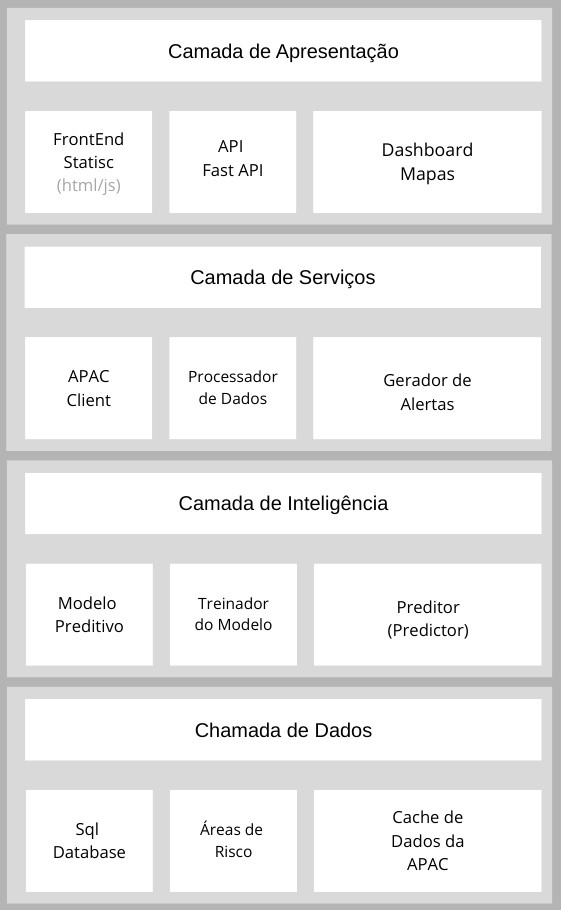
\includegraphics[width=0.9\textwidth]{figuras/estrutura-projeto.png}
    \caption{Arquitetura detalhada do sistema de monitoramento}
    \label{fig:arquitetura-detailed}
\end{figure}


\subsection{Padrões Arquiteturais Aplicados}

A arquitetura segue boas práticas de engenharia de software, como separação em camadas (apresentação, aplicação, domínio e infraestrutura) e princípios SOLID. Isso garante que cada serviço tenha uma responsabilidade única, seja extensível e mantenha interfaces consistentes.

\section{Implementação Técnica}

\subsection{Estrutura de Diretórios e Organização do Código}

A organização do código segue padrões modernos, com separação entre módulos de dados, banco de dados, modelos de predição, serviços de integração e frontend. Essa estrutura facilita a colaboração e a manutenção do projeto.

\begin{lstlisting}[language=bash,caption={Estrutura de Diretórios do Projeto},label={cod:estrutura}]
alagamentos-recife/
|-- docker-compose.yml        # Orquestracao com Docker
|-- Dockerfile                # Containerizacao
|-- requirements.txt          # Dependencias Python
|-- alagamentos.db            # Banco de dados SQLite
|-- app/                      # Codigo-fonte
|   |-- main.py               # Ponto de entrada da API
|   |-- data/
|   |   `-- areas_risco.py    # Definicao das zonas de risco
|   |-- database/
|   |   `-- database.py       # Configuracao e modelos ORM
|   |-- models/
|   |   |-- predictor.py      # Modelo preditivo
|   |   `-- train_model.py    # Treinamento do modelo
|   |-- services/
|   |   |-- apac_client.py    # Cliente HTTP para APAC
|   |   `-- data_processor.py # Logica de ETL
|   `-- static/
|       |-- index.html        # Frontend estatico
|       |-- script.js         # Logica de interface
|       `-- style.css         # Estilos CSS
`-- tests/                    # Casos de teste
\end{lstlisting}

\subsection{Integração com a API da APAC}

Um dos pontos centrais do sistema é a integração com a API da APAC, que fornece os dados meteorológicos em tempo real \cite{alves_apac}. Para isso, foi implementado um cliente especializado que realiza chamadas assíncronas, trata falhas de conexão e garante que o sistema continue funcionando mesmo em caso de indisponibilidade temporária da API. Esse mecanismo de resiliência é fundamental para que os alertas não sejam interrompidos em momentos críticos.
